\chapter{Introduction}\label{sec:intro}
\begin{flushright}{\slshape    
The most important contribution of management in the 20th century\\
was to increase manual worker productivity fifty-fold.\\
The most important contribution of management in the 21st century\\
will be to increase knowledge worker productivity\\
— hopefully by the same percentage} \\ \medskip
--- Peter Drucker~\cite{drucker1999}
\end{flushright}

When Peter Drucker became aware that the automation of manual labour was progressing faster than that of knowledge work, he said these words at the end of the $20^{th}$ century in 1999. Between both types of work lies a pronounced difference: The course of manual work is determined by physical laws, is often very structured and thus offers great potential for easy automation. Knowledge work requires one to "think for a living" and is thus shaped by the individuality of the knowledge worker. As each worker has a different knowledge background and uses information differently, this type of work is very flexible and often no process is ever executed exactly the same. This flexibility incurs making many decisions, as small as they may be - all need to be made by the knowledge worker based upon information. A popular example of a knowledge worker is an insurance company employee who handles multiple insurance claims. Each claim is different, since the information contained in each differs.

Now, 20 years later, numerous knowledge repositories and assistance systems for knowledge workers exist, helping make decisions more informed and faster. From these systems, logs can be extracted which document the course of a process instance from its beginning to its completion. Instances of a process are referred to as cases in the following.

These logs are a valuable source of data as they can reveal best practices that knowledge workers use in certain situations. If this data were processed, such best practices could be recommended by an auxiliary system or the case management system itself. These knowledge worker assistance systems have been called for multiple times in recent literature reviews~\cite{hauder2014, francescomarino2018}, but have only been implemented prototypically until now.

One of the challenges that lie in the way of creation of such a system is the task of anticipating the development of a case, especially that of the next activity. In this area, we want to make a contribution to ongoing research by applying predictive analytics on process execution logs. The result will be an approach with which to predict the next-step of an incomplete case through the use of the case history, as \autoref{fig:next-activity-prediction} shows. This next step could then be processed further by the aforementioned assistance system, e.g. to intervene if a case takes the wrong course.\\

\begin{figure}
    \centering
    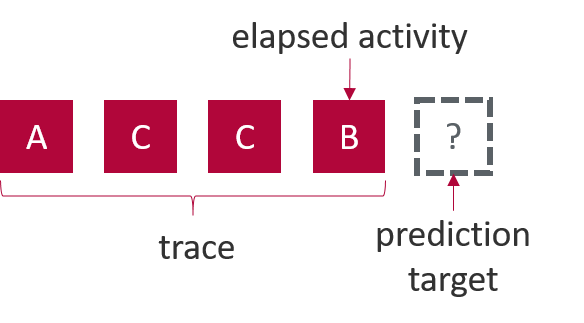
\includegraphics[width=\textwidth]{gfx/next-activity.png}
    \caption{Predicting the next activity, TODO replace}
    \label{fig:next-activity-prediction}
\end{figure}

The application of Predictive Analytics in Process Science is fairly new, and is now commonly referred to as Predictive Process Monitoring. A preliminary definition is delivered along with comprehensive information in \autoref{chap:background}. Furthermore this chapter provides information on Predictive Model Development as well as details on the inner workings of the used type of neural networks.

Then, \autoref{chap:related-work} gives an overview of current approaches to the prediction task at hand, highlighting the achievements and technicalities of each publication. Furthermore it presents work that was done on the problem of sequence prediction in the unrelated field of Natural Language Processing (NLP).

While working with the literature, we realized that the ongoing research in this young domain of Predictive Process Monitoring is lacking in three areas:

\begin{enumerate}
    \item The prediction approaches are not easily comparable, as the published performance measures are based on different datasets. There is only a tendency to make use of the datasets of the Business Process Intelligence Competition (BPIC)~\cite{BPIC2011, BPIC2012, BPIC2017}.
    \item Low technical depth of the publicized approaches makes it unnecessarily hard to reproduce the published results.
    \item A case log is essentially a sequence, but little inspiration has been taken from NLP, where sequence prediction is common.
\end{enumerate}

\marginpar{Maybe we can also use 2016/2017 and give a recommendation what might be a good dataset?\dots}
We want to address these shortcomings in \autoref{chap:contribution} by proposing a revised prediction model that was inspired by predictive models applied in the area of Natural Language Processing (NLP) and stems from injecting engineered features on an intermediate network layer. The approach is tested on the datasets of BPIC 2011 and 2012 and compared to two implementations reverse-engineered from the following publications, thus allowing for a direct comparison:

\begin{enumerate}
    \item \textit{A Deep Learning Approach for Predicting Process Behaviour at Runtime} by Evermann et al.~\cite{evermann2016} \item\textit{Deep Learning Process Prediction with Discrete and Continuous Data Features} by Schönig et al.~\cite{schoenig2018}.
\end{enumerate}

Over the course of reverse-engineering the comparison models and the subsequent evaluation, widely divergent understandings and approaches with regard to the structure of sequential data input for neural networks were uncovered. To contribute to a better understanding in this area, a comparison of the perceived possibilities was incorporated into the evaluation. These findings are presented along with implementation details and performance measures in \autoref{chap:evaluation}.

The thesis ends with \autoref{chap:conclusion}, which summarizes the findings and the accomplishments of this work that began in September 2018. Furthermore it gives pointers with which to improve and continue the work in this active field.